\documentclass[11pt]{exam}
\usepackage[spanish]{babel}
\usepackage[utf8]{inputenx}
\usepackage{fontenc}
\usepackage{textcomp}
\usepackage{lmodern,pifont}
\usepackage{graphicx}
\graphicspath{ {./images/} }
\usepackage{setspace}
\usepackage[dvipsnames]{color}
\usepackage{colortbl}
\usepackage{caption}
\usepackage{amsmath}
\usepackage[normalem]{ulem}

\newcommand\titexam[1]{\centering%
\fbox{\parbox{\textwidth}{\huge \sffamily \textbf{#1}}}\normalsize \vspace{1em}}

\newcommand\materia[1]{%
\parbox{\textwidth}{ \Large \sffamily \textbf{\uline{#1}}}\vspace{1em}}


\newcommand\nombrefecha{%
Nombre y apellidos:\hrulefill
Fecha:\rule{3.5cm}{0.4pt}\vspace{0.5em}}

\renewcommand{\solutiontitle}{\noindent\textbf{Solución:}\par\noindent}
\pagestyle{empty}
\begin{document}
{\fontfamily{lmss}\selectfont

  %%%%%%%%%%%%%%%%%%%%%%%%%%%%%%%%%%%%%
  %% 
\titexam{MF1479\_2 Propagación de plantas en vivero}

\nombrefecha

\materia{Aspectos básicos de botánica y ecofisiología vegetal}
\begin{questions}
\question El nombre científico de una especie se forma de dos partes. ¿Puedes
indicar a que categoría taxonómica corresponde la primera parte?
\begin{checkboxes}
  \choice A. Al Reino
  \choice B. A la Família
  \CorrectChoice C. Al Género
  \choice D. Ninguna es correcta
\end{checkboxes}

\question ¿Sabes que terminación han de tener los taxones pertenecientes a la
categoría de la familia?
\begin{checkboxes}
  \CorrectChoice A. -aceae
  \choice B. -phyta
  \choice C. -ota
  \choice D. La categría de familia no necesita terminación
\end{checkboxes}

\question Señala cuale de las siguientes especies son coníferas
\begin{checkboxes}
  \choice A. Plataneros, encinas y robles
  \choice B. Pinos, cedros y abetos
  \choice C. Enebros, sabinas y cipreses
  \CorrectChoice D. Las respuestas B y C son correctas
\end{checkboxes}

\question ¿En que categoría generalmente están las plantas que al frotar sus
  hojas, estas desprenden un agradable olor?
  \begin{checkboxes}
    \choice A. Plantas olorosas
    \CorrectChoice B. Plantas aromáticas
    \choice C. Plantas perfumadas
    \choice D. Plantas de rosa
  \end{checkboxes}

\question ¿Qué ecosistemas son extremadamente sensibles a la contaminación por
  plantas invasoras y con las que hay que hay que extremar precauciones?
  \begin{checkboxes}
    \choice A. Ecosistemas de montaña
    \CorrectChoice B. Ecosistemas ede agua dulce (rios y sus
    riveras, lagos, humedales, etc)
    \choice C. Ecosistemas dunares
    \choice D. Ecosistema forestal
  \end{checkboxes}
\newpage
\question ¿Qué tipo de raíz aparece en la imagen?
  \begin{figure}[h!]
    \centering
    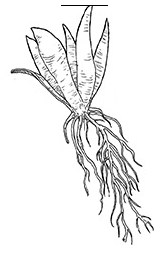
\includegraphics[width: 0.5\textwidth]{./img_/fasciculada.PNG}
  \end{figure}
  \begin{checkboxes}
    \choice A. Napiforme
    \choice B. Pivotante
    \choice C. Ramificada
    \CorrectChoice D. Fasciculada
  \end{checkboxes}

\question ¿Como se llama la parte del tallo a partir de la cual se pueden
  desarrollar flores o tallos?
  \begin{checkboxes}
    \CorrectChoice A. Yemas
    \choice B. Nudos
    \choice C. Lenticelas
    \choice D. Ninguna respuesta es correcta
  \end{checkboxes}

\question ¿Como se llama la parte que une la hoja con el tallo?
  \begin{checkboxes}
    \choice A. Lamina o limbo
    \choice B. Yema axilar
    \CorrectChoice C. Peciolo
    \choice D. Nervadura
  \end{checkboxes}

\question ¿Como se llama la parte de la flor donde se forma y almacena el polen?
  \begin{checkboxes}
    \choice A. Caliz
    \CorrectChoice B. Estambre
    \choice C. Tubo polínico
    \choice D. Gineceo
  \end{checkboxes}

\question ¿Cuales son los factores ambientales que influyen en el desarrollo de
  cultivos?
  \begin{checkboxes}
    \CorrectChoice A. Temperatura, radiación e iluminación, altitud, precipitación,
    velocidad del viento
    \choice B. Topografía, orientación, climatología, frio, calor
    \choice C. Temperatura, iluminación
    \choice D. Altitud y precipitaciones
  \end{checkboxes}
\end{questions}}
\end{document}
%%% Local Variables:
%%% mode: latex
%%% TeX-master: t
%%% End:
